\chapter{Approach}

{In the following, we will present an approach that carries out genetic programming on the basis of a program provided by the expert. The program will be improved so that it makes the same decisions as the black box. The changes to the original program should only include the most necessary and show the expert the most manageable extensions with which he can improve his program.}


\section{General Approach} [TODO need name ]

The approach starts from the point of view of a developer who has dealt with a problem (e.g. Mountain Car) in detail and has already written a program to solve it.
Although the program is already very mature, there is a parallel Reinforcement Learning solution that performs better than the expert's program. This solution is considered a black box and can thus not be explained.
The Expert's program is now to be modified with genetic programming in such a way that it performs just as well as the black box, but still remains close enough to the expert program to allow the developer to recognize the necessary changes.


\begin{figure}[ht]
    \centering
    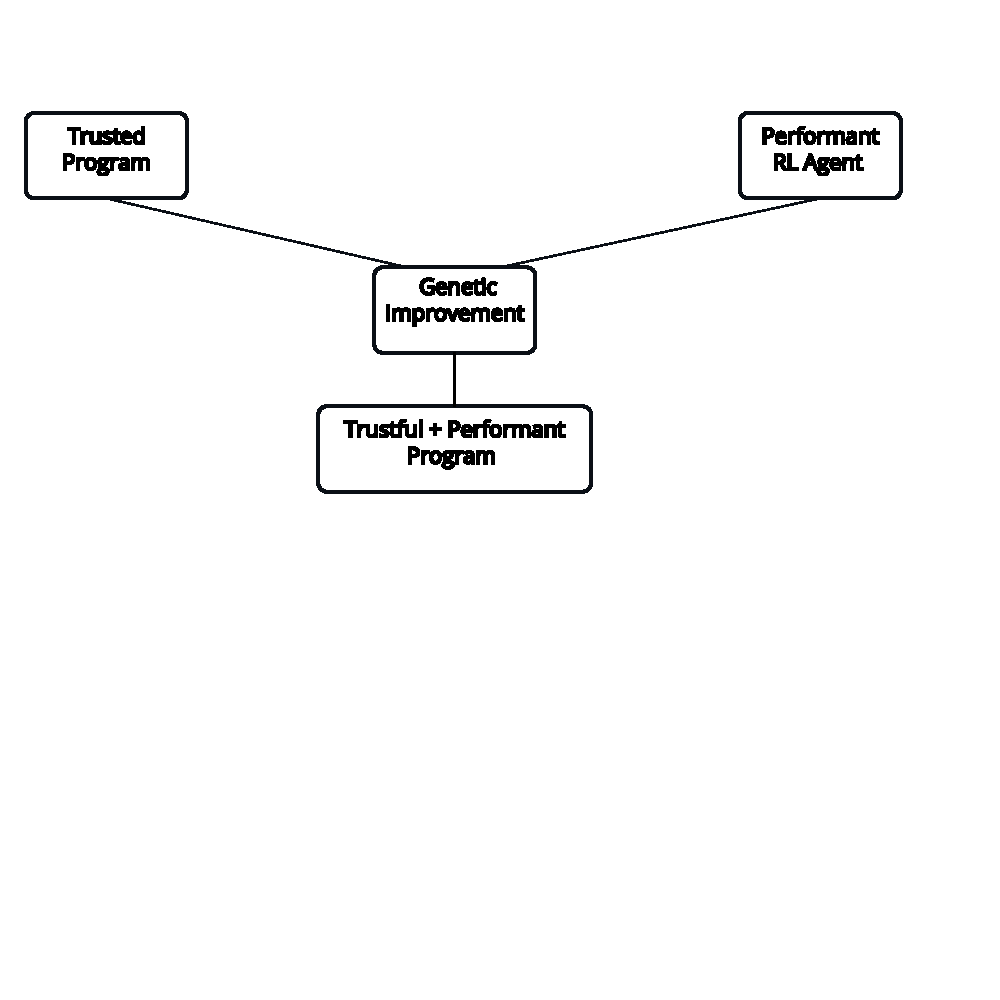
\includegraphics[scale=0.8]{img/plausibility-concept.pdf}
	\caption{TODO, tikz. Combining two known approaches}
	\label{img:plausibility-concept}
\end{figure}

Three components are required:

\begin{enumerate}
% todo graphic
    \item Experts reference solution. A relatable scheme which an expert created with the hope to represent some core logic in form of programming code. This core solution sets the fundamental logic to solve the problem and is the reference of what the developer considers as logical. This will further be called the ``origin'' or ``reference'', as all improvements have its source in this particular part of code.
    It should be noted that this already excludes some problems for which there is no sensibly structured expert programme. Image recognition, for example, is a case that may seem simple, but is still far too complex to be written down as a heuristic.
    \item Best performing ``black box'' solution: A solution that outperforms all other approaches which has to be explained.
    \item Plausible improvements. A genetic programming framework has to improve the hand-written code to the level of the Machine-learning solution while letting the developer understand the changes and where the most substantial improvements can be made.
\end{enumerate}

\subsection{Applicability of the approach}

Proper machine learning problems are those where a certain logic is assumed to be explainable, meaning there is a chance that an expert could define a scheme for an extraordinary well performing solution.\\
This includes:
\begin{itemize}
    \item reinforcement learning approaches
    \item scientific problems
    \item ...
\end{itemize}

This excludes especially those programs that require an extremely high heuristic complexity, for example image recognition with convolutional neural networks. Even though there is a logic in extracting features and matching patterns, the amount of features that need to be extracted is so high that it is nothing a human could explain how it works.\\

\subsection{Why use neural networks as intermediate step?}
Mapping a neural network with genetic programming seems dull at first sight. One could argue that the use of neural networks is superfluous as a solution could as well be optimized solely with genetic programming. While the approach to be applied online [TODO erklärung] is also possible, there are some reasons we want to use them nevertheless.
\begin{itemize}
    \item Faster and better solutions:\\
    By providing a logical foundation, the problem was already separated in core features the programmer has identified. At least, we will further assume that these features do roughly expose the core features of the problem. We will further assume, that more complex or fine features were not found yet.
    \item Offline learning:\\
    We have the possibility to improve our program offline.\\
    Genetic programming also has a different style of converging to a solution. Each generation has multiple candidates that undergo both random and reasonable changes which can lead to good and bad solutions. The candidates can be evaluated parallel, which gives genetic programming an immense speedup. During this process, large rates of  candidates can make decisions that can be very bad.
    
    For example, a good candidate might undergo a tiny change- a '$<$'-sign gets replaced with '$>$'. This will reverse all the good results to bad decisions. Genetic programming is no option for online learning on delicate environments. It is also no option if parallelization is not an option. neural networks are also not a ``good'' option, but still much better than genetic programming.
    \item Even broader range of successful approaches.
    
    Even though genetic programming experiences more popularity, neural networks are much more diverse. For various types of problems, using a specific neural network can confidentially converge so a solution. Some networks have characteristics (that a talented user knows) which perfectly fits thee needs for the problem of choice. In genetic programming, the architecture is generally always the same (consisting of selection, mutation and crossover). Adjustments can only be made by exchanging the operator list or customizing the ratio of genetic operators. The advantage is mostly within the possibility to parallelize everything within a generation.
    \item fine granular changes
    
    \item Crossing approaches
    
    The black box 
    \item No better solution.
    
    One purpose of this work is to explain a specific black box approach. This is why we need to consider exactly what it does.
    \item No solution is also a solution.
    
    If the building blocks we gave the genetic programming approach are not sufficient to find a better solution, the developer can consider the case that no simple annexes to the origin exist. This should not be considered as proof at all, as genetic programming can not guarantee to find  the best or even a good candidate. If solutions are found with much larger complexity or without any logical restriction from the origin or another function set, the expert can identify errors in reasoning that he might not have thought about yet.
\end{itemize}



\section{todo Genetic programming}

Genetic programming (GP) is an evolutionary machine learning approach that can automatically generate and improve programs to solve a problem.
For this purpose, the best programs are selected from randomly generated candidates of a population. The selected candidates can be mutated and crossed to become better and better over generations.

\subsection{TODO Genetic Generations, populations}

The goal of GP is to find the one program over many generations that is better than all the others. To find this program, the population of programs must both promote the best programs and create space for new approaches. (todo Exploration-exploitation tradeoff?) For this purpose, both the selection and the genetic modifications must be chosen accordingly.

\subsection{TODO2 Genetic Selection (Tournament Selection)}
    
In order to achieve a continuous improvement, the programs are evaluated and their fitness is calculated. The best candidates for the next generation are then evaluated through a selection process.

A common way to combine these two approaches is tournament selection. 

A tournament is formed from a handful of candidates (often $3-7$), from which the fittest candidate for the next population is chosen.
This way, even programs that have a poor fitness but may contain genes that will help them survive in the future.

\begin{lstlisting}
n: tournament size
choose n candidates from population
select best candidate
\end{lstlisting}

\subsection{TODO Genetic Mutation}
    
During the mutation, parts of programs are changed.

Point Mutation: A single node of a tree is selected and changed. If the node is a function, it is randomly replaced by a new one. If it is a variable, its value is genetically optimized, for which purpose it is changed with a Gaussian filter.

Branch Mutation: A random node of the tree is selected and the complete branch is regenerated. This allows even larger changes to occur. Furthermore, depending on the length of the new branch, the total number of nodes can either increase or decrease.


\begin{figure}[ht]
	\centering
  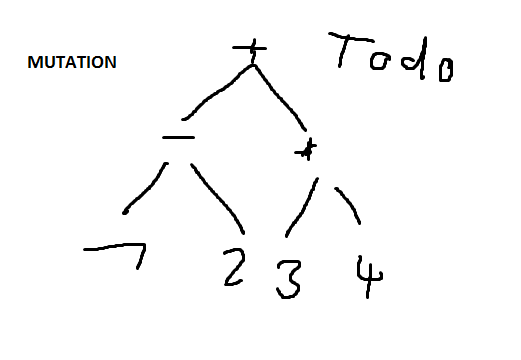
\includegraphics[width=1\textwidth]{img/trees/explain_mutation.png}
	\caption{TODO}
	\label{img:explain_mutation}
\end{figure}

\subsection{TODO Reproduction}
    
    Some good candidates of the last generation can enter the next one without mutation. This is commonly used in genetic programming [todo source].
    Besides, we introduced two additional forms of reproduction:\\
    \begin{itemize}
        \item tes, that are rather close to the origin in the future, without specifically having to reduce the tree-distance between candidates.
        \item Reproduce from 'olymp'. All pareto efficient candidates, including the origin, have a chance to enter the new generation. they are simple and good, its pareto.should be able to give their genes constantly to next gen 
        \item simplify candidates. Either parts of a complete tree gets reduced to the most basic mathematical form possible. Not all trees should be saved in their basic form, as they might have branches with potential for further changes. On the other side, we want simple trees and generally the most basic solution.
    \end{itemize}

\subsection{TODO Genetic Crossover}
    
Candidates can recombine themselves by exchanging their Genes to create children. 

\subsection{TODO Function set, Limitations}

The generated programs consist of operators (todo ?functions?), input values and constant values.

\begin{itemize}
    \item functions / Operators: The set of mathematical operators that make up the program. Possible operators are [TODO $+, -, *$]. 

    Although theoretically all regular functions of regular programming can be used here, loops have been omitted. Although they are a powerful tool in computer science, they lead to severe optimization problems and evaluation problems.
    
    If while-loop is running endlessly, the program can never come to a result and even with a limited number of repetitions the evaluation can take extremely long.
    

    \item Terminals:
    
    Input values: The amount of possible observations in a problem. 
    
    Variables (optional): Randomly chosen constant values. Beside simple values like \tt{True} or \tt{False} mainly numerical constants are selected.

\end{itemize}

Programs can be displayed as a computational tree. TODO image] These are very memory efficient and their components can be easily recognized and divided. 

\subsection{TODO Complexity threshold}


- Complexity

Although fitness is the main criterion, there is often a maximum size that a candidate may not exceed. Complex trees greatly increase the evaluation time. In addition, above a certain level of complexity, no fundamental improvements are expected to solve the problem. The complexity depends mostly on the number of nodes [todo src], but can also depend on other factors such as the depth of the tree.

\subsection{TODO Type consistancy and evaluation safety}

all functions must create working trees

\input{explainability_features}

\input{plagih_extensions}

\subsection{todo, Explanation based genetic programming}

In addition to the known measures, the classic gp can also be extended by functions in many places to ensure even more explainability.


\subsection{todo Experts reference program: origin based gp}
Every problem we can talk about was already analysed thousands of times by neural networks: The human brain. Developing a code by foot, just thinking about the problem, is a very efficient way to create programs. The human brain is incredibly effective compared to machines. It is equipped with a lot of survival instinct, trained with knowledge assimilated from experience made looking at other problems and experience. Regarding a problem, an expert can instinctively abstract a problem and consider many different types of solution structure. Without the need to test dumb stuff. For Plagih, the handwritten code solution (origin) is the base logic the programmer contributes to the problem. The human generated abstraction of the problem is something that human brains are currently far more capable of than neural networks and also represents an aspect that neural networks are very vulnerable of: overfitting. [todo source]. Humans tend to have an aversion against learning and want so solve the same problem thousands of times. [TODO Mathematiker sind faul]. This leads to the solutions to be very effective. Also, humans can see patterns easily to apply solutions from other areas to this one.

Humans have a risk of overfitting aswell without overfitting. If a solution it once considered as respectively good, the search for other solutions is reduced largely (exploration). Examples can be found looking at mistakes some people make over years without knowing that they did anything wrong. "Was Hänschen nicht lerne, lernt Hans nimmer mehr."\\


It is the origin of our genetic programming approach. All trees will stem from this origin  and the complexity of the solution will be related to the origin.

\subsubsection{todo Constant}
Within this tree, the programmer can also specify parts which shall stay the same within the improvement process. This serves both for the reason that the user can relate better to the proposed solution and to help the genetic programming process to save time, as the proposed logic is assumed to not generally prevent better solutions from occuring.

Another interesting option is to provide an incomplete tree that does not represent a good candidate. It does not even have to be a complete mathematical expression. Especially for problems that might have a structure but are extremely hard to parameterize (for example gym's cart pole balance [TODO ref] can be outlined roughly to help the genetic programming find solutions easier.

\subsection{todo Human based genetic programming}

\begin{itemize}
    \item The first generation should be based on the origin
    \item Creating genetic candidates must offer understandable improvements
    \item The complexity measurement must be a plausible distance to the origin
\end{itemize}

Genetic programming generally is free of bias and thus can create better solutions than humans, as stated in [TODO Source http://geneticprogramming.com/]. While this is obviously true, we want to profit from the biases which the developer assumes and let her take advantage of this.

\subsection{Procedure}

\begin{lstlisting} %[language=python]

load_data
    load data_samples
    load origin_tree
    load operators
first_generation
    for size(generation)
        50% mutate(origin)
        50% create_random(origin)
for gen in generations:
    increase parsimony threshold
    create new_generation
        5%  reproduction (1% normal, 2% olymp, 2% reduced)
        25% point_mutation
        30% branch_mutation
        40% crossover
    gene_pool = all, but delete the ones who are too complex (~ <10%)
    compute gene_pool tree fitness with tensorflow
    update pareto_front
terminate
    display the best tree
\end{lstlisting}

\subsection{todo Tournament selection}

The tournament selection chooses n amount of candidates from a population and returns the fittest. If trees have the same fitness, the first one will be chosen, letting the tournament selection be non-deterministic.

\begin{lstlisting} %[language=python]
n = 3
choose n random candidates (from last population)
return fittest
\end{lstlisting}

\subsection{todo Branch mutation}

Branch mutation replaces one node of the computational tree with a randomly new generated subtree, the branch. It allows the candidate to introduce a completely new, random aspect to the candidate.\\
It also is unsafe regarding the distance measurement. It can both decrease and increase the distance to the origin. This operation therefore had to be treated with caution if we do not want too many trees to exceed the parsimony threshold.

\begin{lstlisting}
old_tree

node = tree.random_modifiable_node()

# Create a random insert branch
insert todo

# Find nodes to delete from the tree
old_branch = tree.get_branch(node)

\end{lstlisting}

\subsubsection{Tree grow method}
Trees can be forced to have a specific construction architecture. One option is to construct them in ``full''-mode. This forced the tree to grow to a chosen level.\\
This option can add complexity to the candidates, what helps in finding more complex solutions. This is something we notably do not want. Instead, we will use the ``grow''-method, which adds nodes by chance.

\subsection{Explainable genetic programming framework}
A core feature of approaching a RL-approach with genetic programming is to find a measurement for how ``complex'' changes to his program code is for the developer to relate to.\\
An easy approach is to just count the amount of operations or the amount of operations needed to get from the original code to the improved one. Even though for a computer, it might not be of great difference, for a human brain the type of operation is much more important. Adding several small values can be identified as minor adjustments to variables where ``if-then-else'' operations fundamentally change the code.\\
Finding the optimal weight for the adjustments is not part of this paper, it shall only be shown that improvements based on one factor can be made.\\

\subsection{TODO Explainable Gp Framework, loading origin}

The reference program is preferably loaded from a breadth-first search arranged list of labels, but depending on your preference, a tree can also be generated from a {.csv} file or a mathematical expression. 

Examples:
\begin{itemize}
\item label list: \tt{['$+$', '$*$', '$\sin$', '$1$', '$2$', '$input_1$']} 
\item expression: \tt{todo}
\item Tree ({.csv})\tt{todo}
\end{itemize}

\subsection{TODO marking the core}

To define the core program you have to select the core nodes. In addition to the label list, you need to specify a modification list, which marks for each node whether it can be modified. The nodes must be changeable without interruption up to the root node.

\subsection{TODO Explainable GP Framework, layer0 mutations}

\begin{figure}
    \centering
    
    \begin{lstlisting}
    # get all fix nodes
    # get all fix nodes with non-fix childs
    # get all non-fix childs
    \end{lstlisting}
    \caption{Pseudocode for getting first layer of modifiable nodes}
    \label{fig:my_label}
\end{figure}

\subsection{Parsimony measurements for trees}

The resulting code can be presented to the developer as written code, expression or tree-visualisation. This is just a matter of taste.

The complexity that is a problem to understand is largely affected on these points:
\begin{itemize}
% todo, do i need a lot of sources here?
    \item length.
    The more elements an expression has, the more complex it is. The sheer length of an expression is probably the most obvious cause of complexity.
    \item difference
    \item structure
    \item patterns.
    Humans tend to recognize patterns easily. This means that both recurrent code elements and already known code are easier to realte to.
    \item function types.
    A special pattern is the function type. Some are easy to relate, for example the basic mathematical operations and some are hard to relate to, for example the $tan$-function.
    \item variable types:
    Variables are better to understand, the more simpler they are. 
    \item number of total changes
    A very complex improvement to a program which sets on just one point is easier to understand than the same amount of changes applied at multiple points.
    %todo grafik für alles
\end{itemize}

We already accepted the pattern of the original program as a main influence. The explainability distance to the potential candidates are  resulted in the following considerations for a complexity measurement.
\begin{itemize}
    \item Total amount of operations\\
    A very easy approach is to just count the amount of operations compared to the original program. The problem we get here is, that possibly a completely different approach to a problem is a possible solution. This would leave the user with an approach, where he [TODO or her?] has to give up on his old code. To reduce this risk, a potential solution is to force genetic crossover with the original heuristic. Besides all other approaches, it seems so make sense to also include a value that is not dependent from relative changes to the original heuristic.
    \item Tree Edit distance: Amount of operations applied to the origin\\
    The amount of operations the genetic programming added to the original heuristic seems to be a very reasonable approach, as it corresponds to the lines of code he has to add to his program. However, computational tree-distances have to be computed to receive a correct measurement. This is a known problem in theoretical information technology and has no easy solutions to it.  \label{tree-difference-operations}
    % TODO: Quelle tree distance
    \item Amount of grouped additions to the origin \label{tree-difference-capsuled}\\
    The explainability value here is the amount of added grouped operations (sections) in the tree, that do not lead to original parts of the program. This is also an intuitive measurement, as it corresponds to the amount of points a developer has to improve within his code. Even complex additions would have a high plausibility if they are capsuled within the tree, which corresponds to a small number of possible complex values. What is especially interesting with this measurement is, that it can be computed relatively easy, especially compared to \ref{tree-difference-operations}.
    \item User-specified weights of operations\\
    For the user, who is certain that his program can be improved, different types of operations have a very large difference in plausibility. Therefore, another measurement might make sense instead of counting the sheer number.
    
    \noindent \item[] Some factors, that were thought of and discarded as not helpful:
    
    \item Tree depth:\\
    Tree depth is said to be a good measurement for complexity of programs. However, as already mentioned in \ref{tree-difference-capsuled}, regarding sheer tree-depth as single factor seems to be a poor approach as a long branch which only appends the computational tree at one point feels much better than numerous appends.
    \item Adding scores in each gp-step\\
    This very simple approach would add a plausibility score for every change it performs to the code. This measurement however does not fulfill the triangle-inequality [todo beweis]. Especially recurrent changes would add up meaningless and also crossover operations would become expensive to a point where they can not be used.
    % TODO: https://en.wikipedia.org/wiki/Metric_(mathematics) triangle inequality steht neben subadditivity
\end{itemize}


\subsection{GP Operators}
Genetic programming approaches:

\subsection{typing (strong typing)}
Genetic programming allows automatic conversion of types from truth-values to numbers and visa versa. However, aiming for good explainability, the framework is strongly typed. Reducing a complex mathematical term to a boolean value is both over complicating terms and gives no real benefits as a conversion can also be achieved by generic operators.


\subsection{TODO sympify tree reduce reduction}

One of the most important ways to simplify trees is to simplify the content they represent as a mathematical expression. The simplification process of a formula is very complex 

There were a few things to keep in mind:

- Fix-nodes must not be affected. If 

- Expressions should always be reduced in the same way if possible. Due to the commutative law, for example, the expression $2+a\cdot 2$ is already simplified. However, it can also be arranged differently, for example as $2\cdot a+2$.

- Reduced expressions must not contain any mathematical illogical bits. With the abundance of mathematical simplifications that exist, if all simplifications are allowed, many special cases arise. These often cannot be evaluated, but even then they are often very unfit and in addition often not explainable.

- nan
- zoo
- inf
- complex numbers

\section{Explainability-unrelated gp framework features}

\subsection{TODO Evaluation, Fitness (tensorflow)}
The most complex part of the improvement process is to compute the fitness of a tree. As proposed in \cite{karooGPpaper}, a significant speedup can be achieved by converting the computational tree to tensors and using gpu-parallelism to retrieve fast runs. Karoo offers only very limited options for genetic programming, what lead to the implementation of numerous extensions:
\begin{itemize}
    \item Strong typing
    \item If-condition, minimum and maximum
    \item ...
\end{itemize}


\subsection{What do we know about the black box?}

A central idea of the consideration 
The functionality of the black box was deliberately ignored that an attentive developer would have considered.\\ 
A core idea of the approach to simplify a black box was that the chosen approach does not need to be analysed. Moreover, everything that is found out about the behavior of the approach that would be directly considered a possible source of error by an attentive and conscientious developer has been deliberately ignored.
Examples of this are:
\subsubsection{Missing actions} 
In his reference program, the expert may exclude certain actions that are used by the black box. Often the neural networks create rather smooth transitions. Thus, the policy can never be completely approximated.
This is often a missing neutral action of ``do nothing'', which neural networks decide to go for in borderline cases, as weights are only adjusted slowly. This can then manifest itself in randomized or partially destructive behavior, since the value of the regression from the two extremes to the neutral element is identically equal, and programs with the same regression error can do the complete opposite in situations.
An example is the [todo ref simple agent], which pushes the car either left or right, but never does nothing. 

\subsubsection{Sample selection}
If the primary goal is to improve performance, samples could be selected from the very best runs only. However, care should be taken here, as the best episodes are often those that are easy to solve from scratch. In contrast, the runs where the black box has the most progress over the agent are really interesting. Also conceivable is a collection of outstandingly solved runs to achieve a fitness improvement. [TODO check this out?]

\subsubsection{Sample outlier problems}
[todo should they be handeled?]

Outliers in a dataset tend to attract the attention of the evolving process.
\begin{itemize}
    \item Improvement, period. No matter how small or irrelevant an improvement is, it is an improvement.
    \begin{itemize}
        \item tournament selection: Trees with this gene survive over the ones without this gene. There is no complexity threshold holding these trees back.
    \end{itemize}

\item Many ways to fit outliers\\
Outliers are characterized by being in a sparse space.
The chance of overfitting is quite high though, fitting a weird pattern randomly on a sparse dataset has a high chance of  

\item Sparse data can easily be fit:\\
Improvement can often be achieved with relatively few effort leaving the program core untouched. Using only a couple of elemental mathematical operations or an if-condition is often enough. On one hand, it supports capsulating the program into more parts, however, the programs tend to make weird overfitting of outliers instead of improving the program.
The core logic needs to fit much more data samples correctly, requiring many nodes to achieve only minor improvements. Taking care of all of them requires a lot of fine tuning and structural changes. 
If an improvement is found, the changes are often fundamental. These improvements are harder to achieve, but the required changes often scale similar to the outliers improvements. As a result, the improvement per node is often quite similar.

\item Capsulated changes

\item overfitting occurs randomly and often.\\
functions can ``accidentally'' fit a sample, improving the regression error by only a few.

\item Crossover dilemma: Quantity over quality: The evolutionary crossover likes to populate a generation with these ``genes''

\begin{itemize}
    \item they do not cause a lot of feature interaction to the rest of the code. making an improvement to the partner likely, even if it is not fundamental.
    \item Small branches are more likely to be passed as a whole each time
    \item Many small changes can accumulate, leaving the 
    \item Crossover does not have complexity measurement. Each node is selected with the same probability, doesn't matter if you weight ``arctan(x)'' thousand times higher than ``-(x)''
\end{itemize}

\item You can not be sure if an outlier is actually important or not


\subsubsection{What data for the regression?}
The decision is taken into consideration with the regression kernel. Should the states come from the expert or the beginner or a mixture?
e.g. chess engine alpha zero (pro)…
\begin{itemize}
    \item Pro: alpha zero matches (especially those that end in a draw) can have excessively long endgames that a beginner would never be able to achieve. These would affect the training process at largest, even though they are pretty straight forward. In Mountaincar, the most relevant situations are the ones where the car is the fastest, leaving only few training data. Also, the decision is actually just depending on a few corridors where the revert-decision is made, everything else is just performing the same action?
    \item Pro: playing against yourself excludes the states emerging from playing silly openings or some blunders a priori
    \item Noob: often does not have an endgame to perfect
    \item combining both can both be the best and worst of both worlds?
\end{itemize}

\end{itemize}



\section{Rating candidates with regression error instead of fitness}


The fitness is the common measurement to rate candidates in a population, which represents the performance of the candidate working online in the real environment (or a simulation).

For all experiments in this thesis, the candidates are rated based on the regression error. The regression error is a distance measure to indicate how well a model can predict the labels of a data set (in our case: perform the same actions as the target program). This seems strange at first sight, as we have an environment where we could also calculate the fitness.  In the domain of RL this is usually the reward.

Both the regression error and the fitness correlate strongly. Nevertheless, the differences in the evaluation process and the importance that can be attached to them is greater than one might think.

The fitness, of course, is the more honest value as it represents the actual performance. The main down side that it is very computation-intensive compared to a regression. In an average run, hundreds of generations with about §~1000§ programs or more have to be evaluated. Above all, it requires a lot of CPU power, which would slow down the framework written for this work to a large extent, as it would slow down the special ability to execute jobs in parallel on the GPU by converting it to a tensorflow graph.



\begin{forest}
  for tree={symbol, rounded corners,draw=black!100, fill=green!20}
  point/.style={coordinate,},
  symbol/.style={draw=black,text height=1.5ex,text depth=.25ex,},
  terminal/.style={symbol,},
  nonterminal/.style={rectangle, symbol, rounded corners,fill=green!20},
  operation/.style={symbol, rounded rectangle,},
  fixnode/.style={draw=black!100, fill=red!20,},
  terminal/.style={rectangle, symbol,draw=black!100, fill=green!20,},
  variable/.style={rounded corners, symbol,draw=black!100, fill=green!20,},
  constant/.style={rectangle, symbol,},
 [{$+$},nonterminal,fixnode[{$-$},nonterminal,fixnode[{$\cdot$},nonterminal[{1},terminal,constant][{2},terminal,constant]][{$\cdot$},nonterminal[{3},terminal,constant][{4},terminal,constant]]][{$-$},nonterminal[{$\cdot$},nonterminal[{5},terminal,constant][{6},terminal,constant]][{$\cdot$},nonterminal[{7},terminal,constant][{8},terminal,constant]]]]
\end{forest}